\documentclass[crop=false]{standalone}

\usepackage[subpreambles=false]{standalone}
\usepackage{import}
\usepackage{graphicx}
\usepackage{subcaption}
\usepackage{tikz}

\begin{document}


\begin{center}
  % \hspace*{-0.08\linewidth}
   
 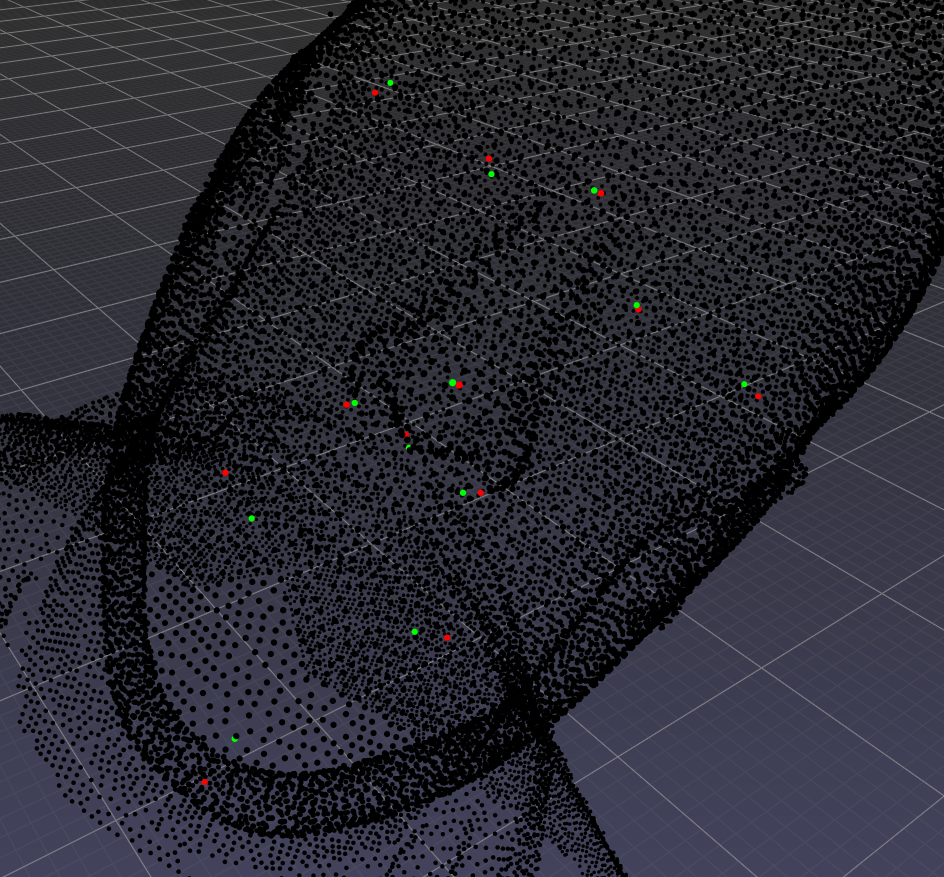
\includegraphics[width=\linewidth]{thesis/results/import/imgs/pred_gt_pt.png}
  %\vspace*{-0.06\linewidth}
 \captionof{figure}{
    \textbf{Result example.}
    \small Initial network predictions (red) against ground truth (green). The ground truth is a manual annotation of a Headspace sample. Sample mean error: 4.40mm. Landmark errors: \mbox{pg = 12.8mm}, \mbox{n = 1.3mm}, \mbox{prn = 1.1mm}, \mbox{ac-r = 1.8mm}, \mbox{sn = 3.4mm}, \mbox{ac-l = 3.3mm}, \mbox{ex-r = 3.8mm}, \mbox{en-r = 3.7mm}, \mbox{en-l = 0.9mm}, \mbox{ex-l = 4.0mm}, \mbox{ch-r = 10.2mm}, \mbox{ch-l = 6.4mm}
  }
  \label{fig:pred_gt_pt}
\end{center}

\end{document}